\chapter{Specifikacija programske potpore}
		
	\section{Funkcionalni zahtjevi}
			
			
			
			\noindent \textbf{Dionici:}
			
			\begin{packed_enum}
				
				\item Neregistrirani korisnik
				\item Klijent				
				\item Iznajmljivač
				\item Administrator

				
			\end{packed_enum}
			
			\noindent \textbf{Aktori i njihovi funkcionalni zahtjevi:}
			


			\begin{packed_enum}
				\item  \underbar{Neregistrirani korisnik može: }
				
				\begin{packed_enum}
					
					\item se registrirati u sustav, stvoriti novi korisnički račun sa svim potrebnim podatcima
					\item  prijaviti se s postojećim podacima za prijavu u sustav
					\item  pregledavati trenutno dostupne romobile i njihove cijene

				\end{packed_enum}
			
				\item  \underbar{Klijent može:}
				
				\begin{packed_enum}
					
					\item pregledavati dostupne romobile
					\item iznajmljivati dostupne romobile te provjeriti je li slike odgovaraju stvarnom stanju
					\item zamijeniti sliku koja ne odgovara stvarnom stanju iznajmljenog romobila novom slikom i kratkim opisom
					\item javiti se iznajmljivaču s porukom i zahtjevom za iznajmljivanje
					\item pregledati povijest svojih transakcija
					
				\end{packed_enum}

				\item  \underbar{Iznajmljivač može: }
				
				\begin{packed_enum}
					
					\item registrirati romobil za što su mu potrebne slike romobila kao dokaz trenutnog stanja
					\item postaviti ponudu za iznajmljivanje i pritom mora unijeti sve relevantne podatke
					\item objaviti na društvenoj mreži o dostupnosti romobila za iznajmljivanje
					\item prijaviti administratoru ako je zamjena slika iznajmljenog romobila predložena bez dobrog razloga
					\item odgovoriti klijentu i prihvatiti ili odbiti ponudu
					\item ocijeniti klijenta i napisati komentar
					\item pregledati povijest svojih transakcija

				\end{packed_enum}

				\item  \underbar{Administrator može: }
				
				\begin{packed_enum}
					
					\item pregledava prijave iznajmljivača i odlučuje hoće li se zamjena slika izvršiti ili ne
					\item pregledava dokumente poslane prilikom registracije te registraciju odobrava ili odbija
					\item zabraniti pristupa svim korisnicima

				\end{packed_enum}

				\item  \underbar{Baza podataka (sudionik) može: }
				
				\begin{packed_enum}
					
					\item pohranjuje sve podatke o korisnicima i njihovim romobilima
					\item pohranjuje sve podatke o transakcijama

				\end{packed_enum}
			\end{packed_enum}
			
			\eject 
			
			
				
			\subsection{Obrasci uporabe}

				
				\subsubsection{Opis obrazaca uporabe}

					

					\noindent \underbar{\textbf{UC1 - Pregled romobila}}
					\begin{packed_item}
	
						\item \textbf{Glavni sudionik: }Neregistrirani korisnik, klijent
						\item  \textbf{Cilj: }Pregledati romobile i njihove cijene
						\item  \textbf{Sudionici: }Baza podataka
						\item  \textbf{Preduvjet: }-
						\item  \textbf{Opis osnovnog tijeka:}
						
						\item[] \begin{packed_enum}
	
							\item Prikazani su dostupni romobili
							\item Korisnik odabire romobil
							\item Prikazuju se informacije i slike romobila te uvjeti za iznajmljivanje

						\end{packed_enum}
					\end{packed_item}
						
					

					\noindent \underbar{\textbf{UC2 - Registracija}}
					\begin{packed_item}
	
						\item \textbf{Glavni sudionik: }Neregistrirani korisnik
						\item  \textbf{Cilj: }Stvoriti korisnički račun za pristup sustavu
						\item  \textbf{Sudionici: }Baza podataka
						\item  \textbf{Preduvjet: }-
						\item  \textbf{Opis osnovnog tijeka:}
						
						\item[] \begin{packed_enum}
	
							\item Korisnik odabire opciju za registraciju
							\item  Korisnik unosi potrebne korisničke podatke
							\item  Sustav provjerava ispravnost podataka
							\item  Korisnik prima obavijest o uspješnoj registraciji
							\item  Sustav preusmjerava korisnika na stranicu s aktivnim oglasima

						\end{packed_enum}
						
						\item  \textbf{Opis mogućih odstupanja:}
						
						\item[] \begin{packed_item}
	
							\item[2.a] Odabir već zauzetog e-maila, unos korisničkog podatka u nedozvoljenom formatu
							\item[] \begin{packed_enum}
								
								\item Sustav obavještava korisnika o neuspjelom pokušaju registracije i vraća ga na stranicu za registraciju
								\item Korisnik mijenja potrebne podatke te završava registraciju ili odustaje od nje
								
							\end{packed_enum}
							
						\end{packed_item}						
					\end{packed_item}



						\noindent \underbar{\textbf{UC3 - Prijava u sustav}}
					\begin{packed_item}
	
						\item \textbf{Glavni sudionik: }Klijent, iznajmljivač, administrator
						\item  \textbf{Cilj: }Dobiti pristup korisničkom sučelju
						\item  \textbf{Sudionici: }Baza podataka
						\item  \textbf{Preduvjet: }Registracija
						\item  \textbf{Opis osnovnog tijeka:}
						
						\item[] \begin{packed_enum}
	
							\item Korisnik odabire opciju za prijavu
							\item Korisnik unosi potrebne korisničke podatke
							\item Sustav provjerava ispravnost podataka
							\item Pristup korisničkim funkcijama

						\end{packed_enum}
						
						\item  \textbf{Opis mogućih odstupanja:}
						
						\item[] \begin{packed_item}
	
							\item[2.a] Neispravni korisnički podatci
							\item[] \begin{packed_enum}
								
								\item Sustav obavještava korisnika o neuspjelom pokušaju prijave i vraća ga na stranicu za prijavu
								
							\end{packed_enum}
							
						\end{packed_item}						
					\end{packed_item}			
					



						\noindent \underbar{\textbf{UC4 - Pregled dokumenata poslanih prilikom registracije}}
					\begin{packed_item}
	
						\item \textbf{Glavni sudionik: }Administrator
						\item  \textbf{Cilj: }Odobravanje ili odbijanje registracije
						\item  \textbf{Sudionici: }Baza podataka
						\item  \textbf{Preduvjet: }Administrator je prijavljen i novi korisnik je registriran
						\item  \textbf{Opis osnovnog tijeka:}
						
						\item[] \begin{packed_enum}
	
							\item Administrator pregledava dokumente poslane prilikom registracije
							\item Registraciju odobrava ili odbija
							\item Odluka dolazi kao obavijest korisniku

						\end{packed_enum}					
					\end{packed_item}	



						\noindent \underbar{\textbf{UC5 - Pregled osobnih podataka}}
					\begin{packed_item}
	
						\item \textbf{Glavni sudionik: }Klijent, iznajmljivač
						\item  \textbf{Cilj: }Pregledati osobne podatke
						\item  \textbf{Sudionici: }Baza podataka
						\item  \textbf{Preduvjet: }Korisnik je prijavljen
						\item  \textbf{Opis osnovnog tijeka:}
						
						\item[] \begin{packed_enum}
	
							\item Korisnik odabire opciju za pregled svojih podataka
							\item Aplikacija prikazuje osobne podatke korisnika

						\end{packed_enum}					
					\end{packed_item}	


						\noindent \underbar{\textbf{UC6 - Promjena osobnih podataka}}
					\begin{packed_item}
	
						\item \textbf{Glavni sudionik: }Klijent, iznajmljivač
						\item  \textbf{Cilj: }Promijeniti osobne podatke
						\item  \textbf{Sudionici: }Baza podataka
						\item  \textbf{Preduvjet: }Korisnik je prijavljen
						\item  \textbf{Opis osnovnog tijeka:}
						
						\item[] \begin{packed_enum}
	
							\item Korisnik odabire opciju za pregled svojih podataka
							\item Korisnik odabere opciju za promjenu podataka
							\item Korisnik mijenja svoje osobne podatke
							\item Korisnik sprema promjene
							\item Baza podataka se ažurira


						\end{packed_enum}
						
						\item  \textbf{Opis mogućih odstupanja:}
						
						\item[] \begin{packed_item}
	
							\item[3.a] Neki podatci nisu popunjeni
							\item[] \begin{packed_enum}
								
								\item Sustav javlja da nisu uneseni svi potrebni podaci
								\item Korisnik dodaje potrebne podatke te završava promjenu ili odustaje od nje
								
							\end{packed_enum}
							
						\end{packed_item}						
					\end{packed_item}	


						\noindent \underbar{\textbf{UC7 - Registriranje romobila}}
					\begin{packed_item}
	
						\item \textbf{Glavni sudionik: }Iznajmljivač
						\item  \textbf{Cilj: }Registracija novog romobila
						\item  \textbf{Sudionici: }Baza podataka
						\item  \textbf{Preduvjet: }Korisnik je prijavljen
						\item  \textbf{Opis osnovnog tijeka:}
						
						\item[] \begin{packed_enum}
	
							\item Korisnik odabire opciju za registriranje romobila
							\item Korisnik popunjava tražena podatke
							\item Korisnik sprema promjene
							\item Baza se ažurira


						\end{packed_enum}
						
						\item  \textbf{Opis mogućih odstupanja:}
						
						\item[] \begin{packed_item}
	
							\item[2.a] Nisu popunjena sva polja obrasca
							\item[] \begin{packed_enum}
								
								\item Sustav javlja da nisu uneseni svi podaci
								\item Korisnik dodaje potrebne podatke te završava registraciju ili odustaje od nje

								
							\end{packed_enum}
							
						\end{packed_item}						
					\end{packed_item}	






						\noindent \underbar{\textbf{UC8 - Postavljanje ponude za iznajmljivanje}}
					\begin{packed_item}
	
						\item \textbf{Glavni sudionik: }Iznajmljivač
						\item  \textbf{Cilj: }Stvoriti novu ponudu za iznajmljivanje romobila
						\item  \textbf{Sudionici: }Baza podataka
						\item  \textbf{Preduvjet: }Korisnik je prijavljen i romobil je registriran
						\item  \textbf{Opis osnovnog tijeka:}
						
						\item[] \begin{packed_enum}
	
							\item Korisnik odabire opciju za stvaranje nove ponude
							\item Korisnik popunjava potrebne podatke
							\item Korisnik sprema promjene
							\item Baza se ažurira


						\end{packed_enum}
						
						\item  \textbf{Opis mogućih odstupanja:}
						
						\item[] \begin{packed_item}
	
							\item[2.a] Nisu popunjena sva polja obrasca
							\item[] \begin{packed_enum}
								
								\item Sustav javlja da nisu uneseni svi podaci
								\item Korisnik dodaje potrebne podatke te završava ponudu ili odustaje od nje

								
							\end{packed_enum}
							
						\end{packed_item}						
					\end{packed_item}	





						\noindent \underbar{\textbf{UC9 - Objavljivanje ponude na društvenoj mreži}}
					\begin{packed_item}
	
						\item \textbf{Glavni sudionik: }Iznajmljivač
						\item  \textbf{Cilj: }Objava na društvenoj mreži o dostupnosti romobila za iznajmljivanje
						\item  \textbf{Sudionici: }Baza podataka
						\item  \textbf{Preduvjet: }Korisnik je prijavljen i postoji ponuda za iznajmljivanje
						\item  \textbf{Opis osnovnog tijeka:}
						
						\item[] \begin{packed_enum}
	
							\item Korisnik odabire oglas
							\item Korisnik objavljuje na društvenoj mreži o dostupnosti romobila za iznajmljivanje


						\end{packed_enum}						
					\end{packed_item}	



						\noindent \underbar{\textbf{UC10 - Kontaktiranje iznajmljivača}}
					\begin{packed_item}
	
						\item \textbf{Glavni sudionik: }Klijent
						\item  \textbf{Cilj: }Podnošenje zahtjeva za iznajmljivanje romobila
						\item  \textbf{Sudionici: }Baza podataka
						\item  \textbf{Preduvjet: }Klijent je prijavljen i postoji romobil za iznajmljivanje
						\item  \textbf{Opis osnovnog tijeka:}
						
						\item[] \begin{packed_enum}
	
							\item Klijent odabire romobil koji želi iznajmit
							\item Klijent se javlja iznajmljivaču s porukom i zahtjevom za iznajmljivanje


						\end{packed_enum}						
					\end{packed_item}	




						\noindent \underbar{\textbf{UC11 - Prihvaćanje ponude}}
					\begin{packed_item}
	
						\item \textbf{Glavni sudionik: }Iznajmljivač
						\item  \textbf{Cilj: }Odluka o iznajmljivanju romobila
						\item  \textbf{Sudionici: }Baza podataka
						\item  \textbf{Preduvjet: }Iznajmljivač je prijavljen i postoji zahtjev za iznajmljivanje
						\item  \textbf{Opis osnovnog tijeka:}
						
						\item[] \begin{packed_enum}
	
							\item Iznajmljivač pregledava zahtjev za iznajmljivanje romobila
							\item Iznajmljivač ga prihvaća ili odbija
							\item Odluka dolazi kao obavijest klijentu


						\end{packed_enum}						
					\end{packed_item}	



						\noindent \underbar{\textbf{UC12 - Iznajmljivanje romobila}}
					\begin{packed_item}
	
						\item \textbf{Glavni sudionik: }Klijent
						\item  \textbf{Cilj: }Najam romobila i provjera odgovaraju li slike romobila stvarnom stanju
						\item  \textbf{Sudionici: }Baza podataka, iznajmljivač
						\item  \textbf{Preduvjet: }Klijent je prijavljen i iznajmljivač je potvrdio zahtjev
						\item  \textbf{Opis osnovnog tijeka:}
						
						\item[] \begin{packed_enum}
	
							\item Klijent izvršava plaćanje 
							\item Klijent provjerava je li romobil odgovara slikama iz ponude


						\end{packed_enum}						
					\end{packed_item}	




						\noindent \underbar{\textbf{UC13 - Zamjena slike romobila}}
					\begin{packed_item}
	
						\item \textbf{Glavni sudionik: }Klijent
						\item  \textbf{Cilj: }Zamjena neodgovarajuće slike romobila sa novom slikom i kratkim opisom što je drugačije na slici
						\item  \textbf{Sudionici: }Baza podataka
						\item  \textbf{Preduvjet: }Klijent je prijavljen i iznajmio je romobil
						\item  \textbf{Opis osnovnog tijeka:}
						
						\item[] \begin{packed_enum}
	
							\item Klijent odabire sliku koju želi zamijeniti
							\item Klijent učitava novu sliku i opis što je drugačije
							\item Klijent sprema promjene
							\item Baza se ažurira


						\end{packed_enum}
						
						\item  \textbf{Opis mogućih odstupanja:}
						
						\item[] \begin{packed_item}
	
							\item[2.a] Nisu popunjena sva polja
							\item[] \begin{packed_enum}
								
								\item Sustav javlja da nisu uneseni svi podaci
								\item Korisnik dodaje potrebne podatke te završava zamjenu ili odustaje od nje

							\end{packed_enum}
							
						\end{packed_item}						
					\end{packed_item}	




						\noindent \underbar{\textbf{UC14 - Prijava pogrešne zamjene}}
					\begin{packed_item}
	
						\item \textbf{Glavni sudionik: }Iznajmljivač
						\item  \textbf{Cilj: }Prijava administratoru da je zamjena slika predložena bez dobrog razloga
						\item  \textbf{Sudionici: }Baza podataka
						\item  \textbf{Preduvjet: }Iznajmljivač je prijavljen i romobil je iznajmljen, izvršena je zamjena slika od strane klijenta
						\item  \textbf{Opis osnovnog tijeka:}
						
						\item[] \begin{packed_enum}
	
							\item Klijent odabire promijenjenu sliku
							\item Klijent odabire prijavu zamjene s kratkim opisom
							\item Klijent sprema promjene
							\item Baza se ažurira


						\end{packed_enum}
						
						\item  \textbf{Opis mogućih odstupanja:}
						
						\item[] \begin{packed_item}
	
							\item[2.a] Nisu popunjena sva polja
							\item[] \begin{packed_enum}
								
								\item Sustav javlja da nisu uneseni svi podaci
								\item Korisnik dodaje potrebne podatke te završava prijavu ili odustaje od nje

							\end{packed_enum}
							
						\end{packed_item}						
					\end{packed_item}	






						\noindent \underbar{\textbf{UC15 - Pregled prijave}}
					\begin{packed_item}
	
						\item \textbf{Glavni sudionik: }Administrator
						\item  \textbf{Cilj: }Odluka o zamjeni slika
						\item  \textbf{Sudionici: }Baza podataka
						\item  \textbf{Preduvjet: }Administrator je prijavljen i podnesena je prijava zamjene slika
						\item  \textbf{Opis osnovnog tijeka:}
						
						\item[] \begin{packed_enum}
	
							\item Administrator pregledava prijave iznajmljivača
							\item Donosi odluku hoće li se zamjena slika izvršiti ili ne
							\item Odluka dolazi kao obavijest i klijentu i iznajmljivaču
							\item Baza se ažurira


						\end{packed_enum}
									
					\end{packed_item}	





						\noindent \underbar{\textbf{UC16 - Ocjenjivanje klijenta}}
					\begin{packed_item}
	
						\item \textbf{Glavni sudionik: }Iznajmljivač
						\item  \textbf{Cilj: }Ocjena klijenta i objava komentara
						\item  \textbf{Sudionici: }Baza podataka
						\item  \textbf{Preduvjet: }Iznajmljivač je prijavljen i romobil je iznajmljen
						\item  \textbf{Opis osnovnog tijeka:}
						
						\item[] \begin{packed_enum}
	
							\item Iznajmljivač odabire klijenta
							\item Dodjeljuje mu ocjenu i piše komentar
							\item Ocjena i komentar se objavljuju na profilu.
							\item Baza se ažurira


						\end{packed_enum}
						
						\item  \textbf{Opis mogućih odstupanja:}
						
						\item[] \begin{packed_item}
	
							\item[2.a] Nisu popunjena sva polja
							\item[] \begin{packed_enum}
								
								\item Sustav javlja da nisu uneseni svi podaci
								\item Korisnik dodaje potrebne podatke te završava ocjenu ili odustaje od nje

							\end{packed_enum}
							
						\end{packed_item}						
					\end{packed_item}	



					\noindent \underbar{\textbf{UC17 - Zabrana pristupa korisnika}}
					\begin{packed_item}
	
						\item \textbf{Glavni sudionik: }Administrator
						\item  \textbf{Cilj: }Zabrana pristupa određenom korisniku
						\item  \textbf{Sudionici: }Baza podataka
						\item  \textbf{Preduvjet: }Administrator je prijavljen
						\item  \textbf{Opis osnovnog tijeka:}
						
						\item[] \begin{packed_enum}
	
							\item Administrator odabire korisnika
							\item Zabranjuje mu pristup aplikaciji
							\item Baza se ažurira


						\end{packed_enum}
						
					\end{packed_item}	



					\noindent \underbar{\textbf{UC18 - Pregled povijesti transakcija}}
					\begin{packed_item}
	
						\item \textbf{Glavni sudionik: }Klijent, iznajmljivač
						\item  \textbf{Cilj: }Pregledati povijest transakcija
						\item  \textbf{Sudionici: }Baza podataka
						\item  \textbf{Preduvjet: }Korisnik je prijavljen
						\item  \textbf{Opis osnovnog tijeka:}
						
						\item[] \begin{packed_enum}
	
							\item Korisnik odabire pregled svojih transakcija
							\item Aplikacija prikazuje povijest transakcija korisnika


						\end{packed_enum}
						
					\end{packed_item}	











				\subsubsection{Dijagrami obrazaca uporabe}
				
				
					\begin{figure}[H]
						\centering
						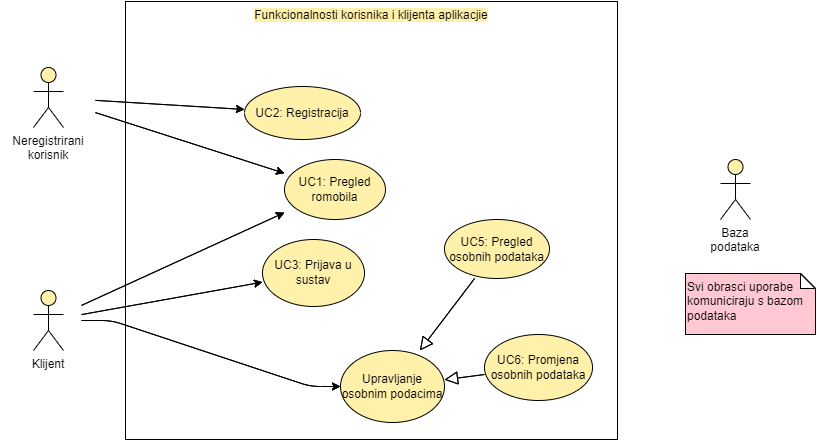
\includegraphics[width=0.8\textwidth]{slike/Funkcionalnost_klijent_korisnik.png}
						\caption{Dijagram obrasca uporabe, funkcionalnost korisnika i klijenta}
						\label{fig:your_label}
					\end{figure}
					
					\begin{figure}[H]
						\centering
						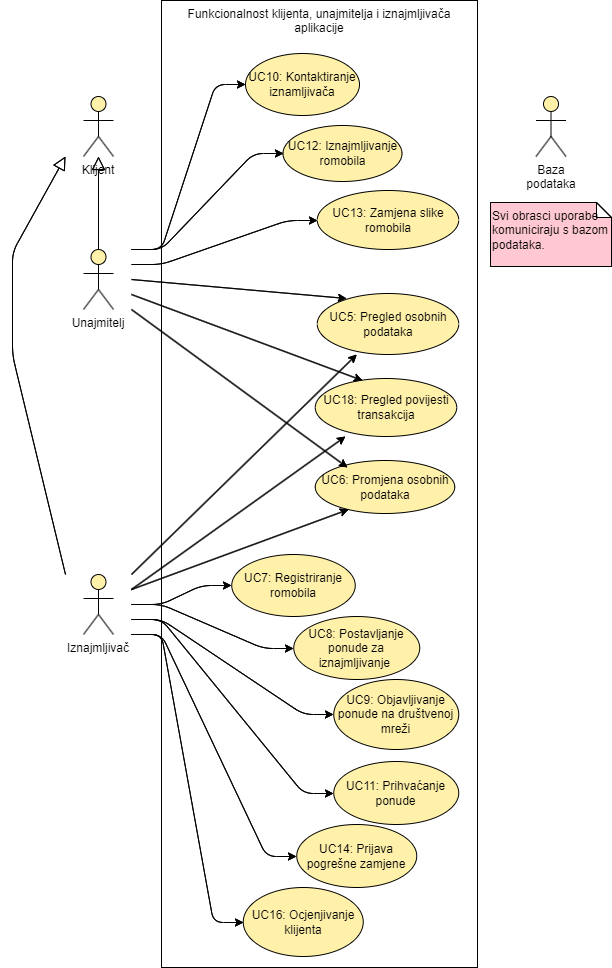
\includegraphics[width=0.8\textwidth]{slike/IznajmljivacUnajmitelj.png}
						\caption{Dijagram obrasca uporabe, funkcionalnost Klijenta, iznajmljivača i unajmitelja}
						\label{fig:your_label}
					\end{figure}
					
					\begin{figure}[H]
						\centering
						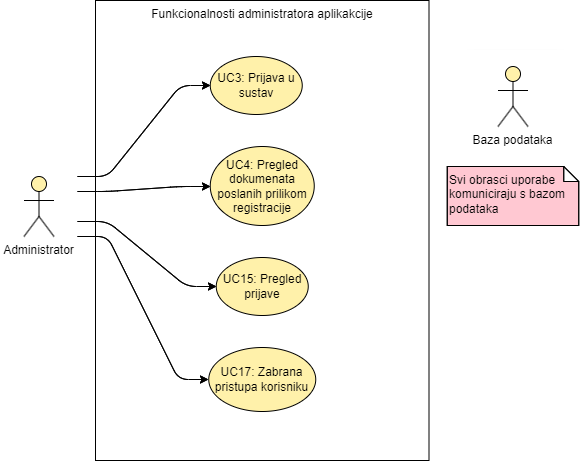
\includegraphics[width=0.8\textwidth]{slike/AdminUC.png}
						\caption{Dijagram obrasca uporabe, funkcionalnost administratora}
						\label{fig:your_label}
					\end{figure}		
				
			\subsection{Sekvencijski dijagrami}
			
				\noindent \textbf{Obrazac uporabe UC15 – Pregled prijave}
				
				\noindent Administrator dobiva obavijest da je iznajmljivača podnio prijavu na zamjenu slika koju je izvršio klijent. Administrator pregledava izmijenjene slike i odlučuje hoće li se zamjena slika izvršiti ili ne. Administratorova odluka dolazi kao obavijest iznajmljivaču i korisniku. Ako je prijava potvrđena nema promjena u bazi, a u slučaju da nije, slike romobila se vraćaju na one prije izmjene.
				\eject
				
				\begin{figure}[H]
					\centering
					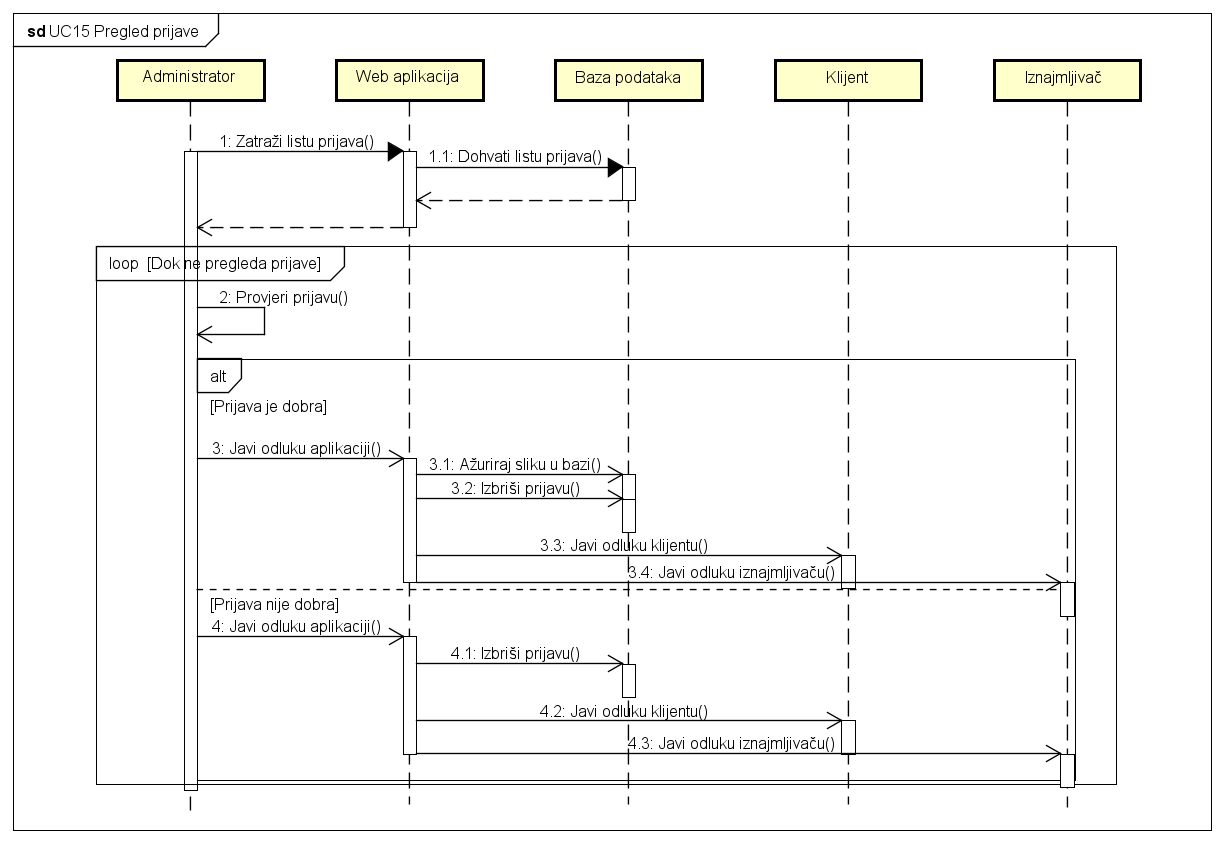
\includegraphics[width=0.8\textwidth]{slike/UC15_Pregled_prijave.png}
					\caption{Sekvencijski dijagram za UC15}
					\label{fig:your_label}
				\end{figure}
				
				\noindent \textbf{Obrazac uporabe UC12 – Iznajmljivanje romobila}
				
				\noindent Klijent inicira zahtjev za pregled dostupnih oglasa kako bi odabrao željeni romobil. Poslužitelj potom pristupa trenutnim oglasima iz baze podataka i prikazuje ih klijentu. Nakon odabira oglasa, poslužitelj povlači sve relevantne podatke o odabranom romobilu i predstavlja ih klijentu. Korisnik ima mogućnost provjeriti usklađenost prikazanih fotografija romobila s njegovim stvarnim stanjem. Kada klijent donese odluku, šalje zahtjev za iznajmljivanje romobila iznajmljivaču. Iznajmljivač ima opciju prihvatiti ili odbiti zahtjev klijenta. U slučaju prihvata, poslužitelj prosljeđuje relevantne podatke o rezervaciji romobila bazi podataka.
				\eject
				
				\begin{figure}[H]
					\centering
					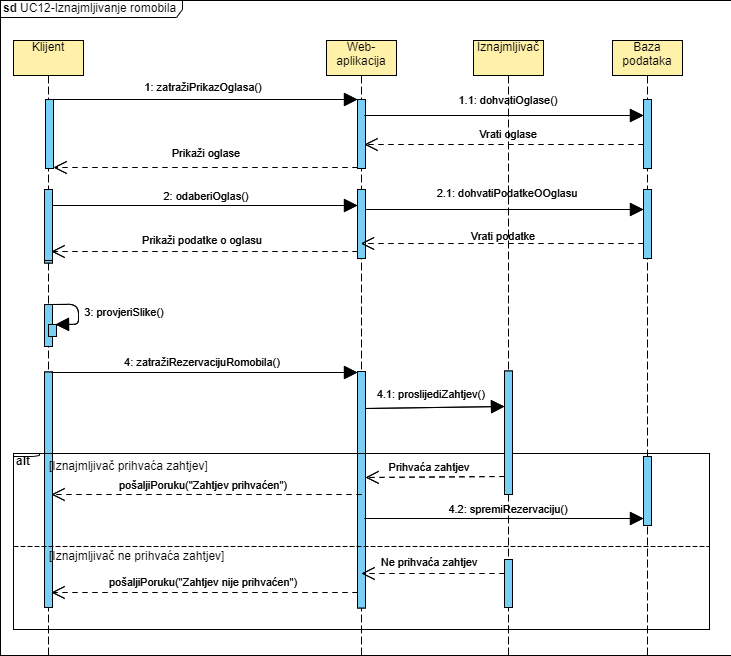
\includegraphics[width=0.8\textwidth]{slike/sd_uc12.png}
					\caption{Sekvencijski dijagram za UC12}
					\label{fig:your_label}
				\end{figure}
				
				\noindent \textbf{Obrazac uporabe UC16 – Ocjenjivanje klijenta}
				
				\noindent Iznajmljivač odabire klijenta kojemu onda on dodjeljuje ocjenu i komentar. Ukoliko nisu popunjena oba polja za ocjenu i komentar, aplikacija iznajmljivaču šalje poruku da nisu uneseni svi podaci te mo daje opciju ponovnog unosa. Tu poruku iznajmljivač dobiva za svaku takvu nepotpunu objavu. Iznajmljivač može tada odustati od objave ili nadopuniti. Ocjena i komentar su nakon toga vidljivi na profilu klijenata.
				\eject
				
				\begin{figure}[H]
					\centering
					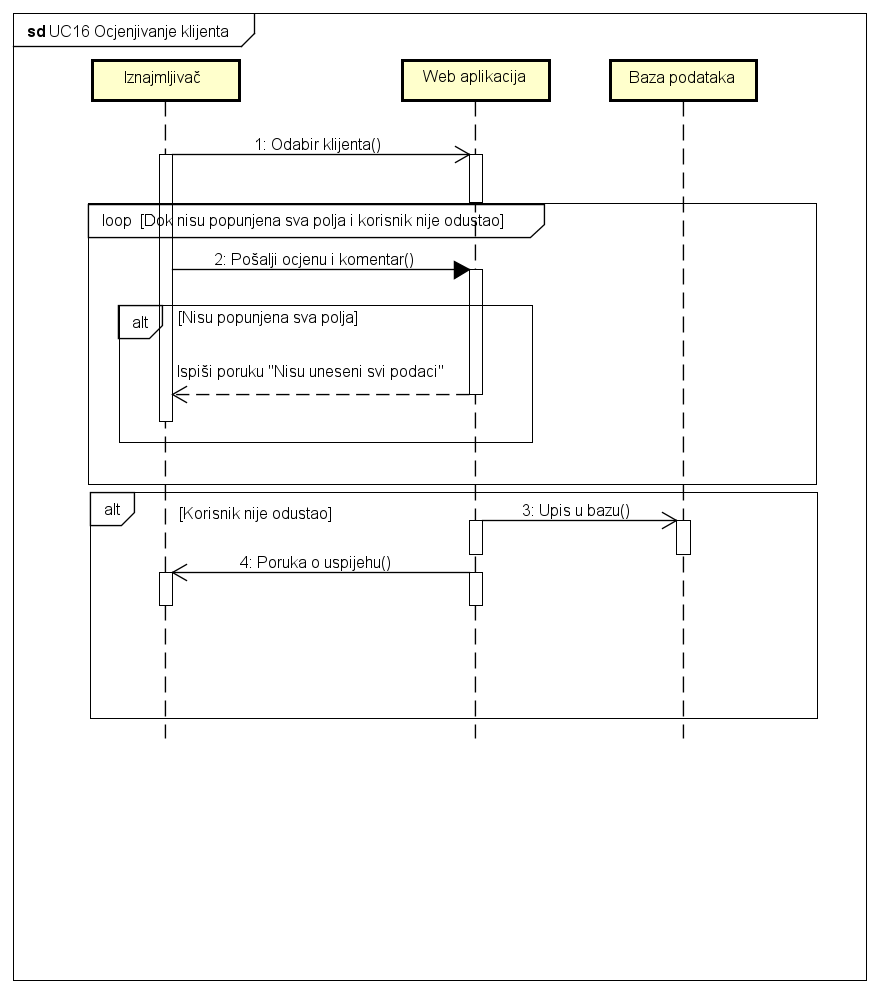
\includegraphics[width=0.8\textwidth]{slike/UC16_Ocjenjivanje_klijenta.png}
					\caption{Sekvencijski dijagram za UC16}
					\label{fig:your_label}
				\end{figure}
	
		\section{Ostali zahtjevi}
		
			\begin{packed_item} 
				\item Sustav treba omogućiti rad više korisnika u stvarnom vremenu
				\item Korisničko sučelje i sustav moraju podržavati hrvatsku abecedu (dijakritičke znakove) pri unosu i prikazu tekstualnog sadržaja
				\item Izvršavanje dijela programa u kojem se pristupa bazi podataka ne smije trajati duže od nekoliko sekundi 
				\item Sustav treba biti implementiran kao web aplikacija koristeći objektno-orijentirane jezike
				\item Neispravno korištenje korisničkog sučelja ne smije narušiti funkcionalnost i rad sustava
				\item
				Sustav treba biti jednostavan za korištenje, korisnici se moraju znati koristiti sučeljem bez opširnih uputa
				\item 
				Nadogradnja sustava ne smije narušavati postojeće funkcionalnosti sustava
				\item 
				Sustav kao valutu koristi EUR
				\item 
				Veza s bazom podataka mora biti kvalitetno zaštićena, brza i otporna na vanjske greške
				\item 
				Pristup sustavu mora biti omogućen iz javne mreže pomoću HTTPS.
			\end{packed_item}
			 
			 
			 
	